%%%%%%%%%%%%%%%%%%%%%%%%%%%%%%%%%%%%%%%%%%%%%%%%%%%%%%%%%%%%%%%%%%%%%%%%%%%%%%%%
% event_selection.tex
%%%%%%%%%%%%%%%%%%%%%%%%%%%%%%%%%%%%%%%%%%%%%%%%%%%%%%%%%%%%%%%%%%%%%%%%%%%%%%%%
\chapter{Analysis Strategy}
\label{analysis}
A key challenge for this type of analysis is the identification of muons without relying on information from the muon chambers, as energy loss from \dbrem may cause signal muons to have large mismatches in the tracker and muon chamber hits or fail to reach the muon chambers at all.
Additionally, muon candidates must be selected with very high purity to eliminate potential backgrounds from misidentified muons which lose energy via decay or standard model showing in insensitive detector material.
Lastly, events must pass one of the available CMS triggers in order to be saved.
If signal muons have significant energy loss from \dbrem they will no longer pass the reconstruction requirements necessary for typical trigger selections, and only events containing alternate particles which do fulfill the trigger selections will be kept.

For these reasons, a tag-and-probe method is used to select events with muon pairs produced in Z decays, with high-quality 'tagging' muons reconstructed with full muon chamber information and passing requirements for CMS muon triggers are paired with 'probe' tracks which are likely to be produced by the other muon from the decay.
By requiring that the tag and probe pair have an invariant mass near the mass of the Z boson and pass several isolation requirements designed to remove non-muon tracks, probe tracks can be selected which have high likelihoods of originating from muons without using information from the muon chambers along their trajectory.

Once probe tracks are selected, they can then be extrapolated into the HCAL and CSCs in order to search for evidence of missing energy that may have been caused by the production of an \aprime.
Signal events are split into two categories based on the presence of nearby standalone muons.
'Complete disappearance' events have no nearby standalone muons, and correspond to events where the track is fully stopped before reaching the muon chambers or suffers a complete reconstruction failure within them.
'Partial disappearance' events have standalone muons nearby to the probe track, but have large energy differences in the reconstructed standalone muon and the selected track.
In the complete disappearance region a simultaneous fit of the invariant mass distribution is made to distinguish signal and DY events from non-muon backgrounds, while in the partial disappearance region a binary decision tree is used to better differentiate potential signal events from background and a single-bin count is made for the final selection.
A sketch of an example complete disappearance event and an example partial disappearance event is shown in \Cref{fig:sigCatSketch}.

\begin{figure}[htpb]
	\centering
	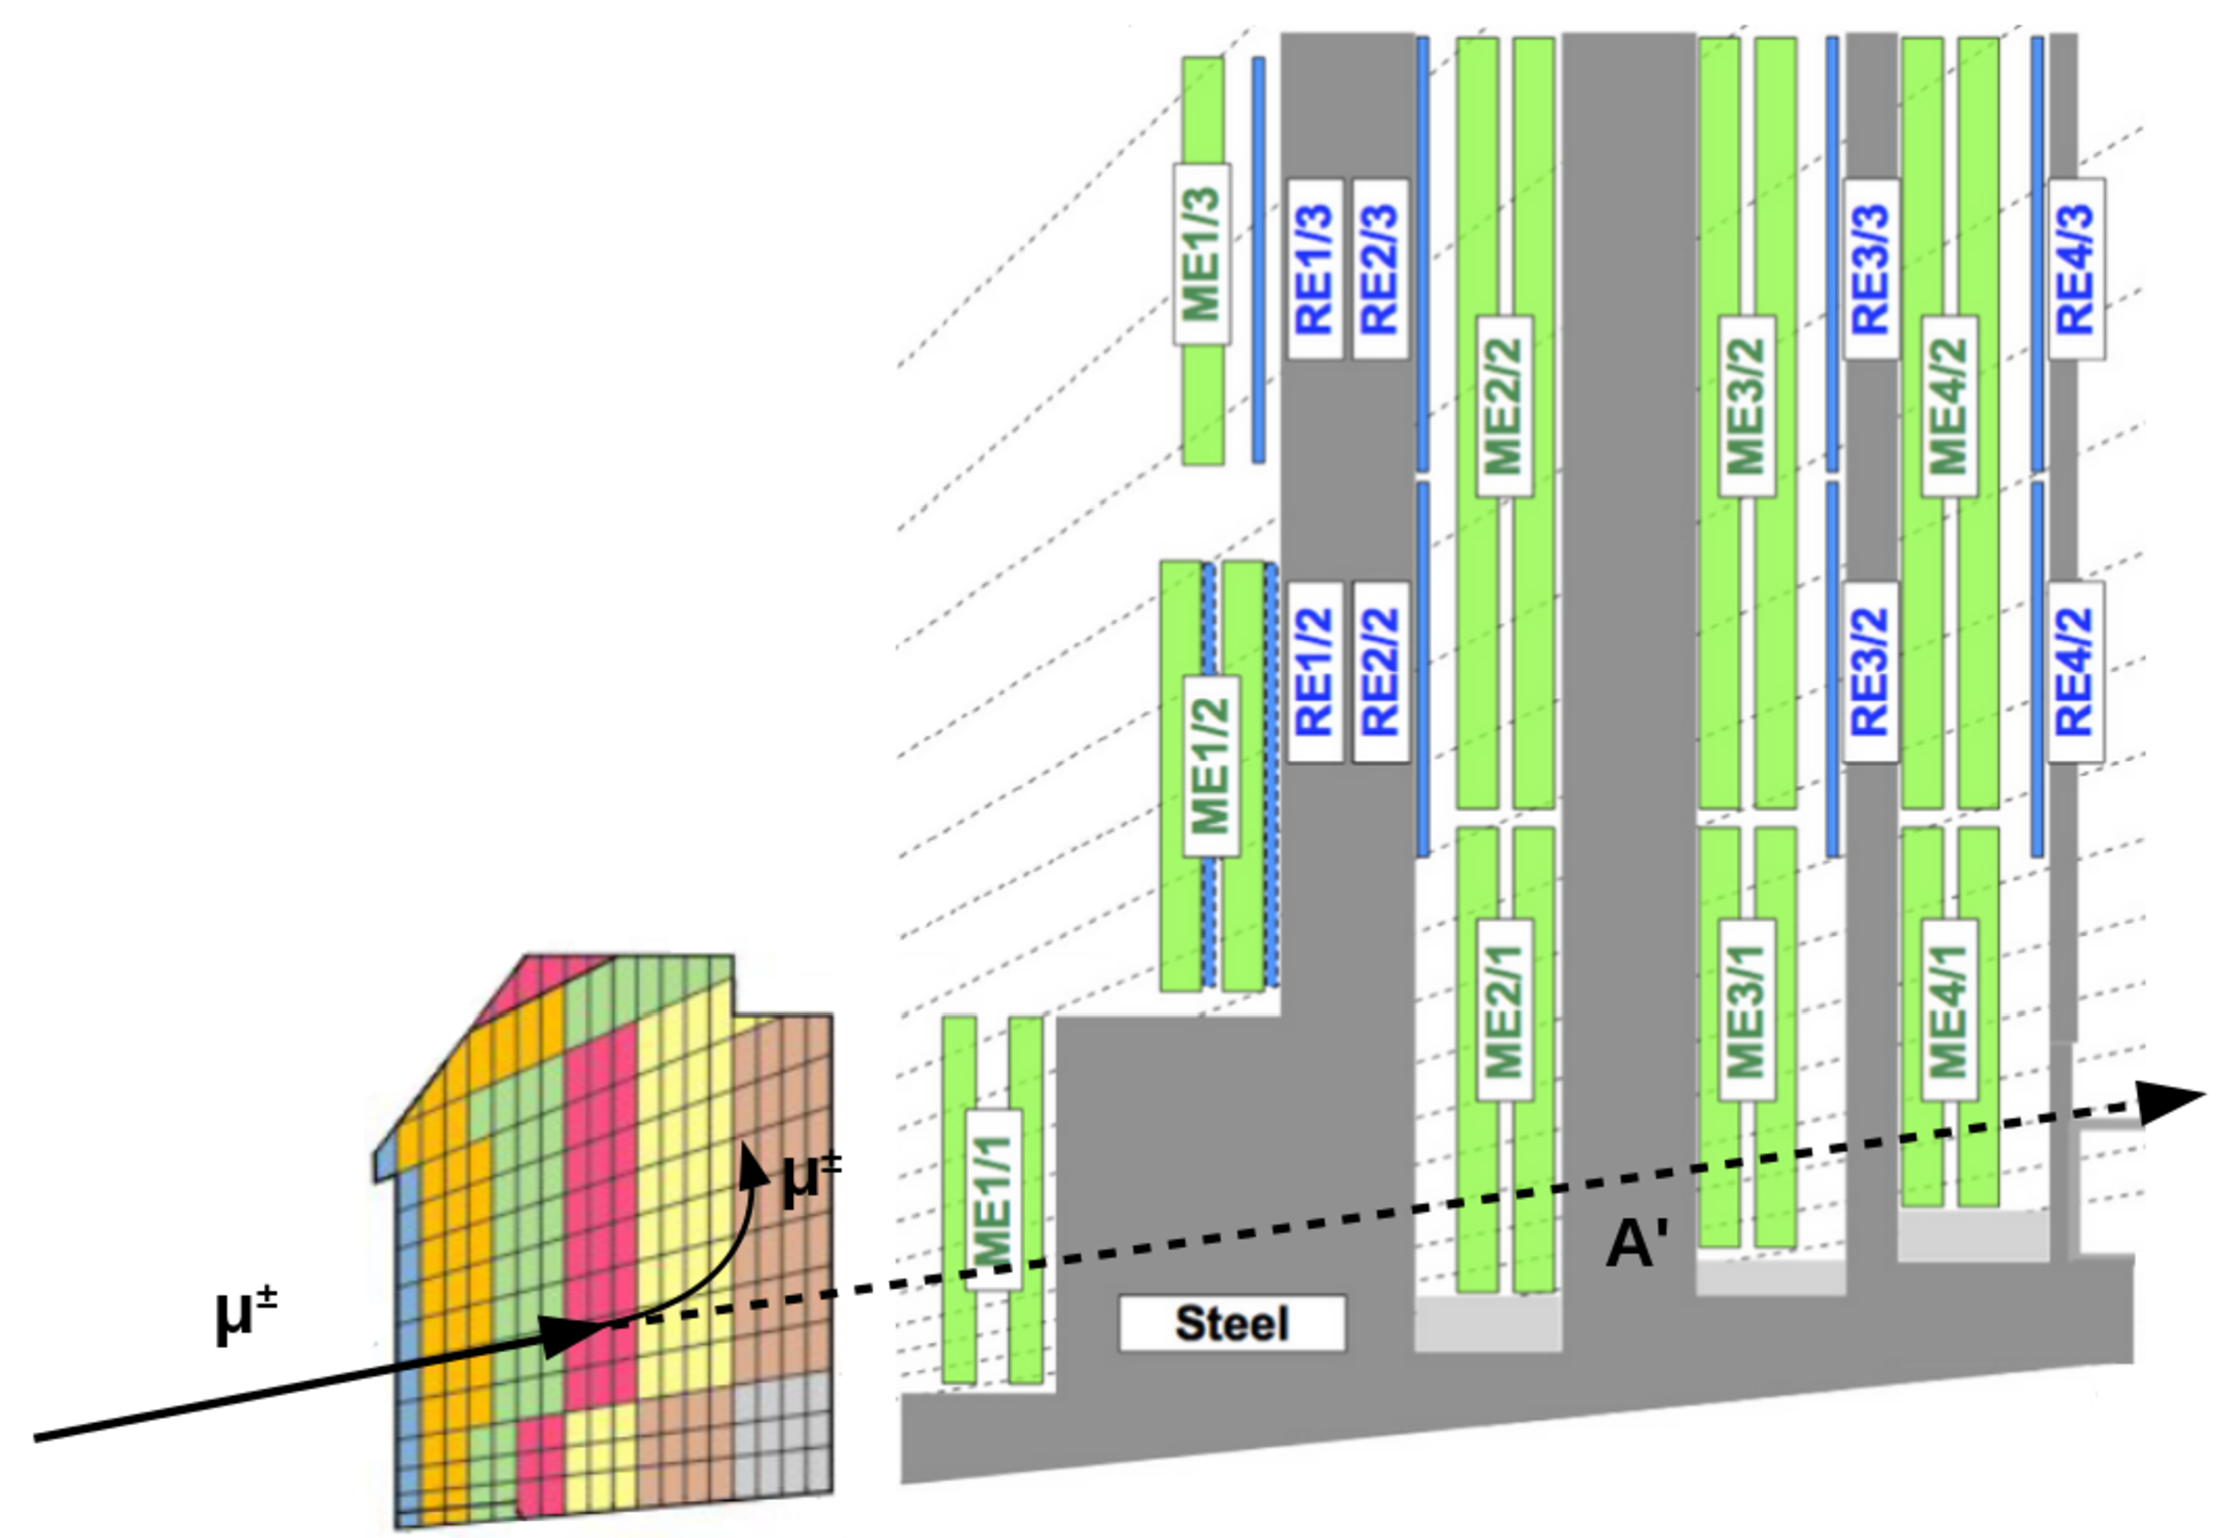
\includegraphics[width=0.45\textwidth]{figures/comp_dis.pdf}
	\hspace{0.01\textwidth}
	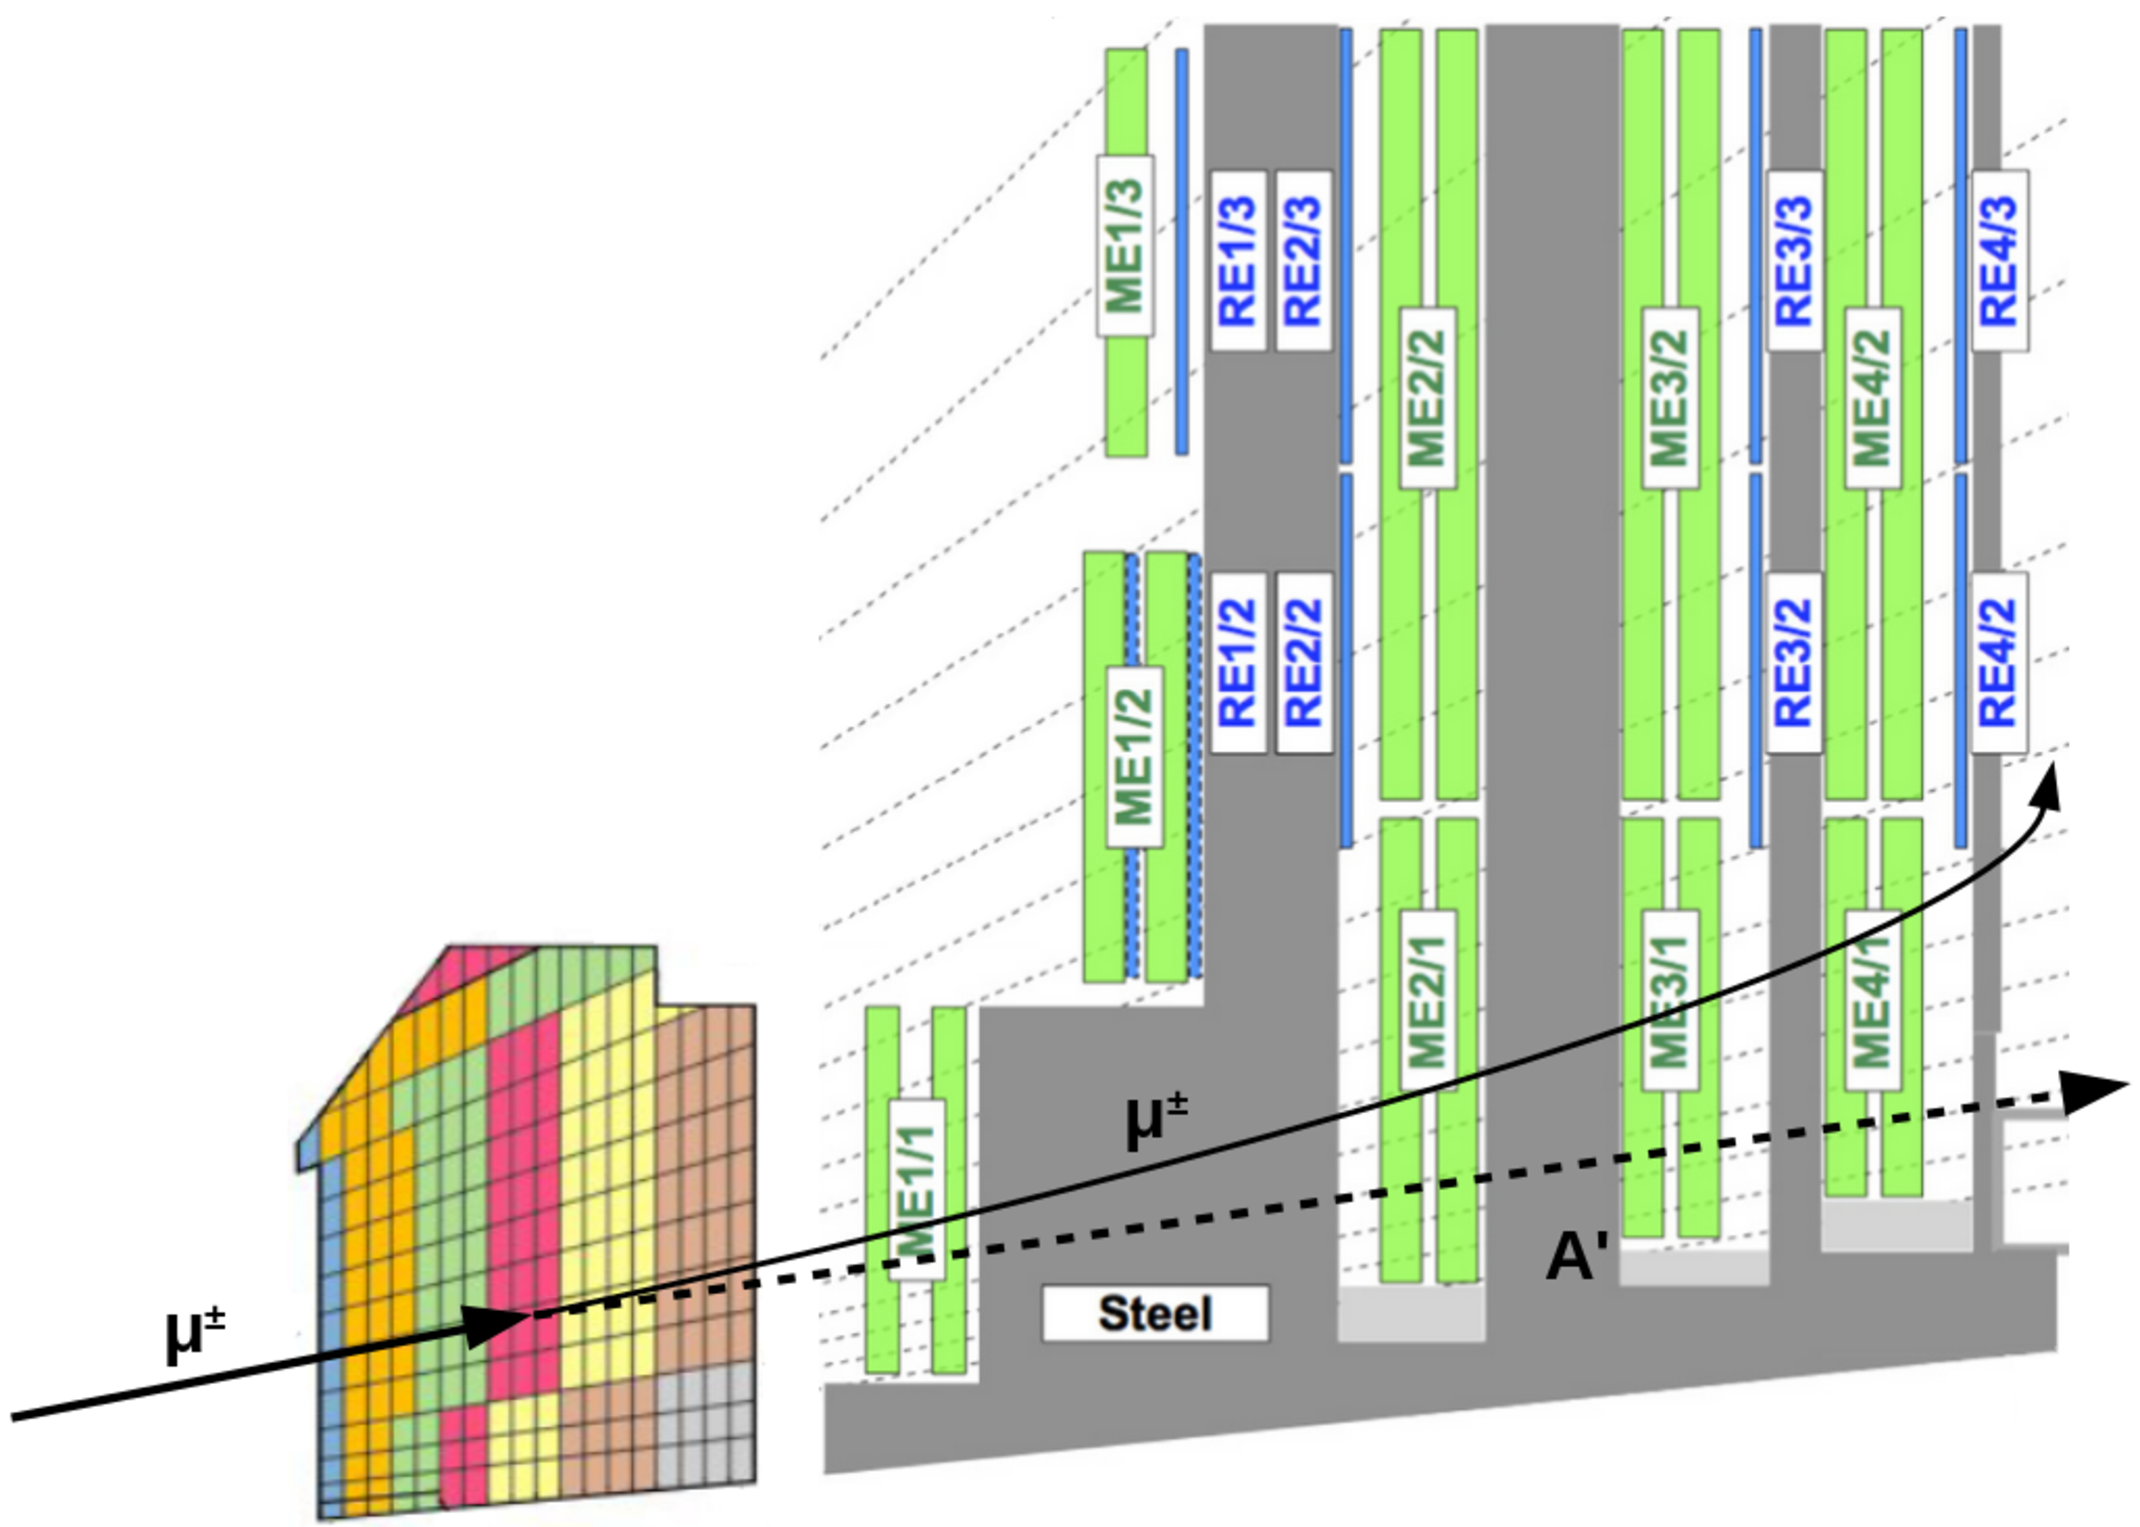
\includegraphics[width=0.45\textwidth]{figures/part_dis.pdf}
	\caption[Example Complete and Partial Disappearance Events]{A representative complete disappearance event (left) and a partial disappearance event (right). In both cases a dark matter interaction produces an A' within the HCAL, while in complete disappearance events the scattered muon has so little energy it does not create a nearby standalone muon and in partial disappearance events a standalone muon is produced with some measureable missing energy.}

\section{Base Event Selection}
The initial process of pairing probe tracks with tagging muons is referred to as the Base Event Selection, and is used in both the signal regions and a variety of control regions.
This definition of a "base event" is also useful for interpreting the final results of the search, when the observed number of signal events is compared to the expected number of background events and the signal sensitivity.
This process initially produces results in terms of an arbitrary 'signal strength', related to the normalization of the signal events, which must be re-interpreted into a meaningful physical quantity.
By measuring the rate at which events which pass the base event selection in MC pass the base event selection at a given cross section and scaling them to the number of base events seen in data, the signal strength can be re-interpreted as the cross section for \dbrem.
Using this method, uncertainties from the CMS collision luminosity, the DY cross section, and the parton distribution functions used can be greatly reduced, as the number of predicted probe tracks would otherwise include the product of those quantities.

The base event selection begins with the tagging muons, used to pass the CMS trigger and to pair with probe tracks to find Z-candidates.
Selected tagging muons are required to have $\eta<$2.4 to be within the fiducial region of the CMS detector. 
As discussed in \cref{sec:muonReco} the tagging muons must be global muons, and have several additional requirements applied to avoid potential fakes from hadronic punch through, cosmic rays, or other processes which could produce ionization in the muon chambers.
The global fit of potential tag muons must have $\chi^2<$10 and include at least one hit from the muon chambers, and the global muon itself must also have muon segments in at least two muon stations.
The inner track of each candidate tagging muon is required to have a transverse (longitudinal) impact parameter $<$\SI{2}{\milli\meter} ($<$\SI{5}{\milli\meter}) to the primary vertex, with at least one pixel hit and six tracker layer hits.

The tagging muons must be isolated from other particles to further reduce backgrounds from non-DY events, wherein muons can frequently be produced within jets of other particles.
The tagging muon isolation is defined as the ratio of the transverse energy of neutral hadrons and photons from pileup plus the transverse momentum of all charged hadrons from the primary vertex minus half the transverse energy of charged hadrons from pileup in a $\Delta$R cone of 0.4 to the transverse momentum of the muon, and it is required to be less than 15$\%$.

Lastly, only tagging muons which pass the requirements for the CMS high-pt, isolated muon trigger are used in order for the correct application of several scale factors applied with the assumption that the tagging muon was the particle which fired the trigger.
The $p_t$ threshold for the CMS isolated muon trigger is \SI{24}{\giga\eV}, and only tagging muons with $p_t>$\SI{26}{\giga\eV} are selected in order to reduce uncertainties related to the efficiency of triggering on muons near the trigger threshold.

Similarly to the tagging muons, the selected probe tracks have several requirements on their kinematics and track quality to reduce backgrounds from non-DY events, with additional requirements in place to reject events with large energy deposits nearby from SM bremsstrahlung.
Probe tracks are required to have \pt$>$\SI{20}{\giga\eV}, and 1.45$<\eta<$2.4 to be within the HCAL endcap.
They must also have $\Delta\mathrm{R}>$0.2 to the tagging muon to explicitly remove events where the probe track and tagging muon originate from the same particle.

Only tracks which pass the 'high-purity' selections in CMS track selection are used, a category which is defined by selections for the minimum number of tracker layers with hits, the maximum number of layers with missing hits, the reduced $\chi^2$ of the resulting fit, and several other requirements relating to the precision with witch the initial vertex position is measured.
The exact values used to define a high-purity track vary depending on the track parameters and several iterations of attempted track fitting, and a full description of the high-purity selection and track fitting process can be found in \cite{trackFitting}.
Lastly, probe tracks are selected to have transverse (longitudinal) impact parameters $<$\SI{0.05}{\milli\meter} ($<$\SI{0.5}{\milli\meter}) to the primary vertex to further reduce the rate of selecting poorly-reconstructed tracks or particles produced after the initial collision.

The probe track must be well isolated within each individual subdetector to remove non-muon backgrounds and events with significant muon scattering from standard model processes. 
The probe tracker isolation, defined as the \pt sum of all other tracks within a $\Delta$R cone of 0.3 originating from the same primary vertex divided by the \pt of the selected track, must be less than 0.05.
In the ECAL, the energy sum of all hits with energy greater than \SI{0.3}{\giga\eV} in a $\Delta$R cone of 0.4 to the probe track must be less than \SI{10}{\giga\eV}.
Similarly, the energy sum of all HCAL hits within a $\Delta$R cone of 0.3 to the probe track must be less than \SI{30}{\giga\eV}. 
As mentioned in \cref{sec:detector}, potential probe tracks must be in the active ECAL and HCAL regions so that these isolation requirements can be effectively applied, with all candidate tracks required to have $\Delta$R$>$0.1 to any known inactive region.

Once the potential tagging muons and probe tracks in an event have been chosen, each track is individually paired with each muon to search for pairs which are likely to originate from Z bosons.
Successful pairs must have oppositely charged tag muons and probe tracks, and be fit using a \kf algorithm to form a shared vertex with reduced $\chi^2<$3.
In the signal region the pair must have an invariant mass between 80 and \SI{100}{\giga\eV} to be near the Z-mass, while several control regions extend this range from 50 to \SI{150}{\giga\eV}.

Once a tag and probe pair is chosen, the pairing of the tagging muon to all other tracks in the event without quality or geometric acceptances is checked for any other potential matches.
Any tagging muons which pass the pairing requirements with these alternate tracks are rejected to remove events where the tagging muon originates from a Z decay but the second muon has a poor track or fails geometric acceptance, potentially allowing a particle track which is un-associated with the Z-decay to be selected as the probe.
Similarly, tagging muons which pass the pairing requirements with any other global muon in the event with $\Delta$R greater than 1.0 to the selected probe track are rejected to reduce background events where the second muon from the Z-decay has a poorly reconstructed track but is still visible in the muon chambers.

\section{Signal Selection}
After using the base event selection to identify tracks which are likely to originate from muons without using the muon chamber information, an additional categorization is made to search for \dbrem-like event features in the further reaches of the detector.
Signal events are categorized into two separate categories based on the presence of nearby standalone muons along the probe track trajectory.
"Complete disappearance" events have no standalone muons reconstructed within $\Delta$R of 1.0 to the probe track, while "Partial disappearance" events have at least one standalone muon within $\Delta$R$<$1.0, with an additional requirement that the highest energy standalone muon within the $\Delta$R cone of 1.0 has at most 40$\%$ of the probe track energy.
Several additional selections are applied to each region to further separate signal from background events.

In the complete disappearance region, the added selections are designed to reduce the rate of backgrounds produced by mis-identified probe tracks or events with large showers within the detector.
Because of the increased rate of non-muon backgrounds in complete disappearance events stronger requirements are placed on the sum of the HCAL energy along the track trajectory, with the selection reduced to $<$\SI{10}{\giga\eV} along the probe track trajectory, optmized using the rate of events far from the Z peak. 
Conversely, a requirement that at least two HCAL cells along the probe trajectory have $>$\SI{0.1}{\giga\eV} is applied to remove events where the probe particle may shower in ECAL or the support structure before reaching HCAL.

In addition to the requirement of no nearby standalone muons, no CSC hits are allowed to be within $\Delta$R of 0.05 to the probe track in order to reject events where mis-identified hadrons or mesons pass through HCAL without fully showering and deposit some energy in the muon chambers, as well as events that may have muon deposits in the CSCs and significant failures in muon reconstruction such that no standalone muons are formed.

In the partial disappearance region, the requirement of a nearby standalone muon greatly reduces the backgrounds caused by mis-identified tracks, and the dominant backgrounds are caused by DY muons with poorly-reconstructed standalone muon energies.
Due to the relatively large uncertainty in standalone muon reconstruction, the requirement that the standalone muon have $<$40$\%$ of the probe track energy still results in $\mathcal{O}(10^{5})$ selected DY muons.
To reduce this background, a binary decision tree is used to separate signal from DY backgrounds, which is described in detail in \Cref{sec:BDT}.
Partial disappearance events are thus required to have 'signal-like' BDT scores of $>$0.98, reducing the expected DY backgrounds by several orders of magnitude.
As the individual HCAL depth energies are used as in input to the BDT, events with probe track trajectories near the edges of and HE cell are rejected to prevent issues from mis-alignment (\Cref{sec:HCALeff}).

In comparisons of candidate partial disappearance events in data with low BDT scores ($<$0.7), an excess of data events with poorly reconstructed standalone muon features was observed.
These events are observed to have large scatters in $\phi$ from the first CSC chamber to the later CSC chambers, an effect which does not appear in signal events but results in anomalously low energy standalone muons.
To reject these events, a standalone muon quality requirement was added which removes events that have large differences in position from the first CSC station to the later three.
To pass the quality selection, partial disappearance events must have $>$1 muon segment in the later three muon stations within $\Delta$R$<$0.05 of the closest muon segment in station one to the projected probe track trajectory.
